%% Semplice beamer conforme al powerpoint ufficiale
%% dal sito di Ca' Foscari. Si basa sul tema "default"
%% mandate Modifiche e migliorie! Guido.Caldarelli@unive.it 
% Elenco Contributori 
% Guido Caldarelli, Matteo Brilli 

%\documentclass{beamer}
% decide below the aspect ratio between 16:9 and 4:3
%\documentclass[aspectratio=43]{beamer}
\documentclass[aspectratio=169]{beamer}

\usepackage[utf8]{inputenc}
\usepackage{tikz}
\usepackage{multicol}
\usetikzlibrary{tikzmark, shapes}
\usepackage{bm}
\usepackage[dvipsnames]{xcolor}
% Questo tema commentato di sotto produce un beamer più tradizionale 
%\usetheme[secheader]{Boadilla}


%%%-----------------------------------------------------------%
%% Cambia colori da thema default
%% Questi sono i due colori ufficiali rosso e grigio
\definecolor {cfred}{rgb}{0.709,0.196,0.329} 	%{ 181 ,50 ,84}
\definecolor {cfgrey}{rgb}{0.537,0.537,0.537} 	%{ 137,137,137}
\definecolor {cflink}{rgb}{0.615,0.615,0.607} 	%{157,157,155}
\definecolor {cfgreen}{rgb}{0.004, 0.196, 0.125} %{1, 50, 32}

\setbeamercolor{palette primary}{bg=cfred,fg=white}
\setbeamercolor{palette secondary}{bg=cfred,fg=white}
\setbeamercolor{palette tertiary}{bg=cfred,fg=white}
\setbeamercolor{palette quaternary}{bg=cfred,fg=white}
\setbeamercolor{palette five}{bg=cfgreen, fg=white}
\setbeamercolor{structure}{fg=cfred}		 % itemize, enumerate, etc
\setbeamercolor{section in toc}{fg=cfred} 		 % TOC sections
% Override palette coloring with secondary
\setbeamercolor{subsection in head/foot}{bg=cfgrey,fg=white}
%%%------------------------------------------------------------

%% Definisce il blocco con riquadro che non è presente nel tema default (commentare se si usano altri temi)
\setbeamercolor{uppercolor}{fg=white,bg=cfred}%
\setbeamercolor{lowercolor}{fg=black,bg=white}%
\def \bblock{\begin{beamerboxesrounded}[upper=uppercolor,lower=lowercolor,shadow=true]}
\def \eblock{\end{beamerboxesrounded}}
%%-----------------------------------------------------------
\setbeamertemplate{footline}[frame number]
\setbeamertemplate{caption}{\raggedright\insertcaption\par}
%% Intestazione ripetuta per ogni slide
\addtobeamertemplate{headline}{%
\vspace{0.25cm} \ \ 

\includegraphics[height=1.0cm]{Ca_Foscari Beamer/cambridge-cropped.pdf}

\includegraphics[height=1.0cm]{kicc.png} 	% sostituire con logobeamIT.png per italiano
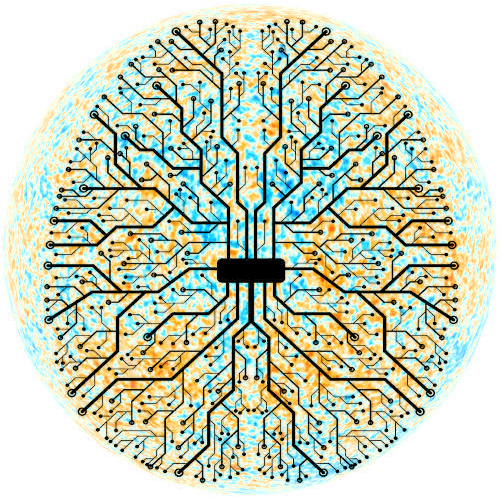
\includegraphics[height=1.0cm]{Ca_Foscari Beamer/handley-lab.png}
%\hspace{0.641\textwidth}{\color{cflink} {\small www.unive.it}} %per 16:9
%\hspace{0.551\textwidth}{\color{cflink} {\small www.unive.it}} %per 4::3
\vspace{0.25cm}
{\color{cfred} \hrule \hrule  }
\textbf{}
}{}
%%-------------------------------------------------------------

%This block of code defines the information to appear in the Title page
%%%
\title[Accelerated nested sampling with $\beta$-flows for gravitational waves] %optional
{Accelerated nested sampling with $\beta$-flows}

\author[Metha Prathaban] % (optional)
{Metha Prathaban \break myp23@cam.ac.uk \break \vfill
\includegraphics[width=0.22\textwidth]{Ca_Foscari Beamer/qr-code.png}}
\date{}

\setbeamertemplate{frametitle}[default][right, rightskip=.5cm] {}
\addtobeamertemplate{frametitle}{\vspace*{-1.4cm}}{}
%End of title page configuration block
%------------------------------------------------------------


%------------------------------------------------------------
%The next block of commands puts the table of contents at the 
%beginning of each section and highlights the current section:

\AtBeginSection[]
{
  \begin{frame}
    \frametitle{Table of Contents}
    \tableofcontents[currentsection]
  \end{frame}
}
%------------------------------------------------------------

\begin{document}

%The next statement creates the title page.
\frame{\titlepage}
%---------------------------------------------------------
%This block of code is for the table of contents after
%the title page
\begin{frame}
\frametitle{About Me}
\begin{itemize}
    \item 3rd year PhD student
    \item Work on Bayesian numerical method development in context of GWs
\end{itemize}
\vspace{2em}
\bblock{\begin{center}
Current work is in collaboration with Will Handley and Harry Bevins.
\end{center}}
\begin{center}
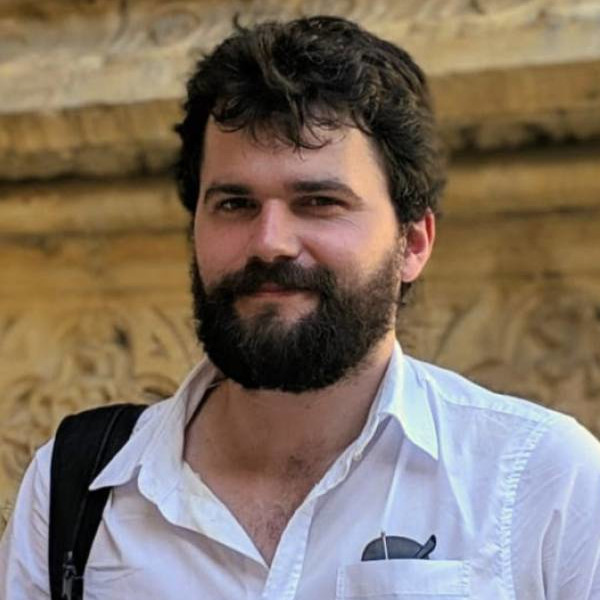
\includegraphics[height=2.0cm]{Ca_Foscari Beamer/will_handley.jpg}

\includegraphics[height=2.0cm]{Ca_Foscari Beamer/harry_bevins.jpg}
\end{center}
\eblock
\end{frame}
%This block of code is for the table of contents after
%the title page
\begin{frame}
\frametitle{Table of Contents}
\tableofcontents
\end{frame}
%---------------------------------------------------------


\section{Nested sampling}


%---------------------------------------------------------
% %Changing visibility of the text
% \begin{frame}
% \frametitle{Bayes' Theorem for Gravitational Waves}
% \begin{minipage}{\textwidth}\vspace{1em}
%     Given some model $\mathcal{M}$ and observed signal $\mathcal{D}$, Bayes' theorem enables us to relate the posterior probability of the set of parameters $\theta$ which generated the signal to the likelihood of the $\mathcal{D}$ given $\theta$ and the prior probability of $\theta$ given $\mathcal{M}$:
% \end{minipage}
% \begin{minipage}{0.22\textwidth}\vspace{0.5em}
% \begin{figure}
% \centering
% 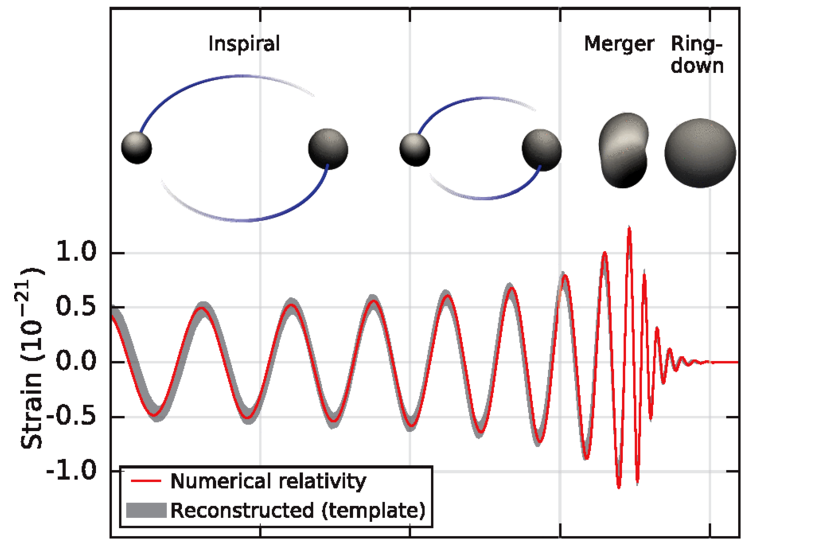
\includegraphics[height=0.95\textwidth]{Ca_Foscari Beamer/Screenshot from 2024-10-14 13-25-30.png}
% \caption{\textcolor{cfgrey}{1602.03837}}
% \end{figure}
% \end{minipage}
% \hspace{30pt}
% \begin{minipage}{0.6\textwidth}
% \centering
% \begin{align*}
%     \mathcal{P}(\theta | D, \mathcal{M}) = \frac{P(D | \theta, \mathcal{M}) P(\theta | \mathcal{M})}{P(D | \mathcal{M})} = \frac{\mathcal{L}(D | \theta)\pi(\theta)}{\mathcal{Z}}
% \end{align*}
% \end{minipage}%
% \vfill
% \begin{minipage}{\textwidth}
% The evidence, $\mathcal{Z}$, plays a key role in model comparison.
% \end{minipage}
% \end{frame}

%-------------------------------------------------------------
% \begin{frame}{Inverse problems in GW physics}
% \begin{columns}
%     \column{0.9\textwidth}
%     \vspace{1em}
%     \centering
%     % \textbf{GW astronomy}
%     % \vspace{0.5em}
%     \begin{figure}
%         \centering
%         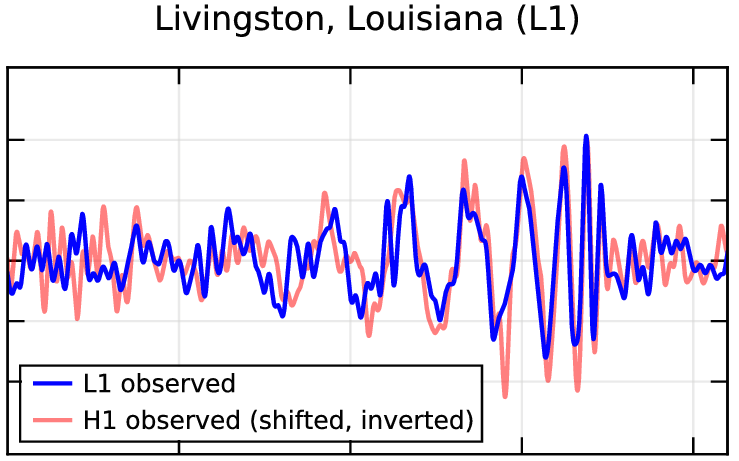
\includegraphics[width=0.4\textwidth]{Ca_Foscari Beamer/gw_example.png.png}
%     \end{figure}
%     \vspace{0.5em}
%     \only<1>{ 
%     \node {\textbf{Forward} : Given a waveform model and a set of binary parameters, \textcolor{red}{model} the GW signal.}
% }%
% \only<2>{ 
% \node {\textbf{Inverse} : From an observed signal strain, $h(t)$, \textcolor{red}{infer} the binary parameters (e.g. masses, spins, luminosity distance, sky location etc.)}
% }%
% \end{columns}
% \end{frame}

%Changing visibility of the text
\begin{frame}{Bayes' Theorem}\vfill
    Given some model $\mathcal{M}$ and observed signal $\mathcal{D}$, Bayes' theorem enables us to relate the \textcolor{RoyalBlue}{posterior} probability of the set of parameters $\theta$ which generated the signal to the \textcolor{Purple}{likelihood} of the $\mathcal{D}$ given $\theta$ and the \textcolor{BurntOrange}{prior} probability of $\theta$ given $\mathcal{M}$:

\vfill
\begin{minipage}{0.3\textwidth}
    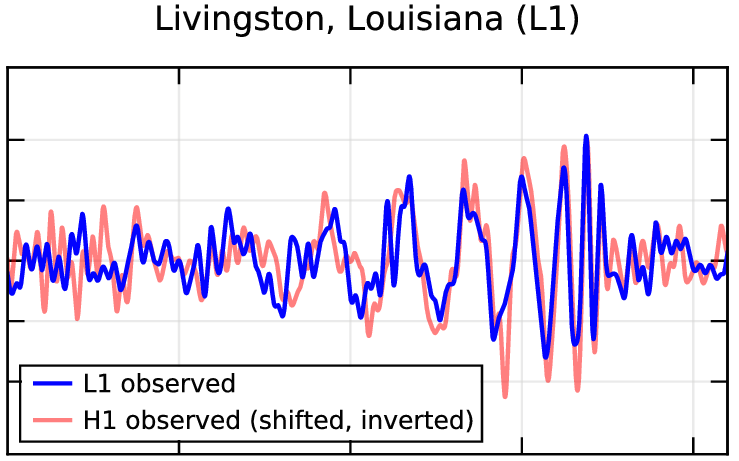
\includegraphics[width=\textwidth]{Ca_Foscari Beamer/gw_example.png.png}
\end{minipage}\hspace{2em}
\begin{minipage}{0.6\textwidth}
\begin{equation}
    \textcolor{RoyalBlue}{\mathcal{P}(\theta | D, \mathcal{M})} = \frac{\textcolor{Purple}{P(D | \theta, \mathcal{M})} \textcolor{BurntOrange}{P(\theta | \mathcal{M})}}{\textcolor{red}{P(D | \mathcal{M})}} = \frac{\textcolor{Purple}{\mathcal{L}(D | \theta)} \textcolor{BurntOrange}{\pi(\theta)}}{\textcolor{red}{\mathcal{Z}}}
\end{equation}
\end{minipage}
\vfill
The \textcolor{red}{evidence}, \textcolor{red}{$\mathcal{Z}$}, plays a key role in model comparison.
\end{frame}

\begin{frame}{Outputs in \textsc{bilby}}
    \begin{minipage}[]{0.5\textwidth}
    \centering
        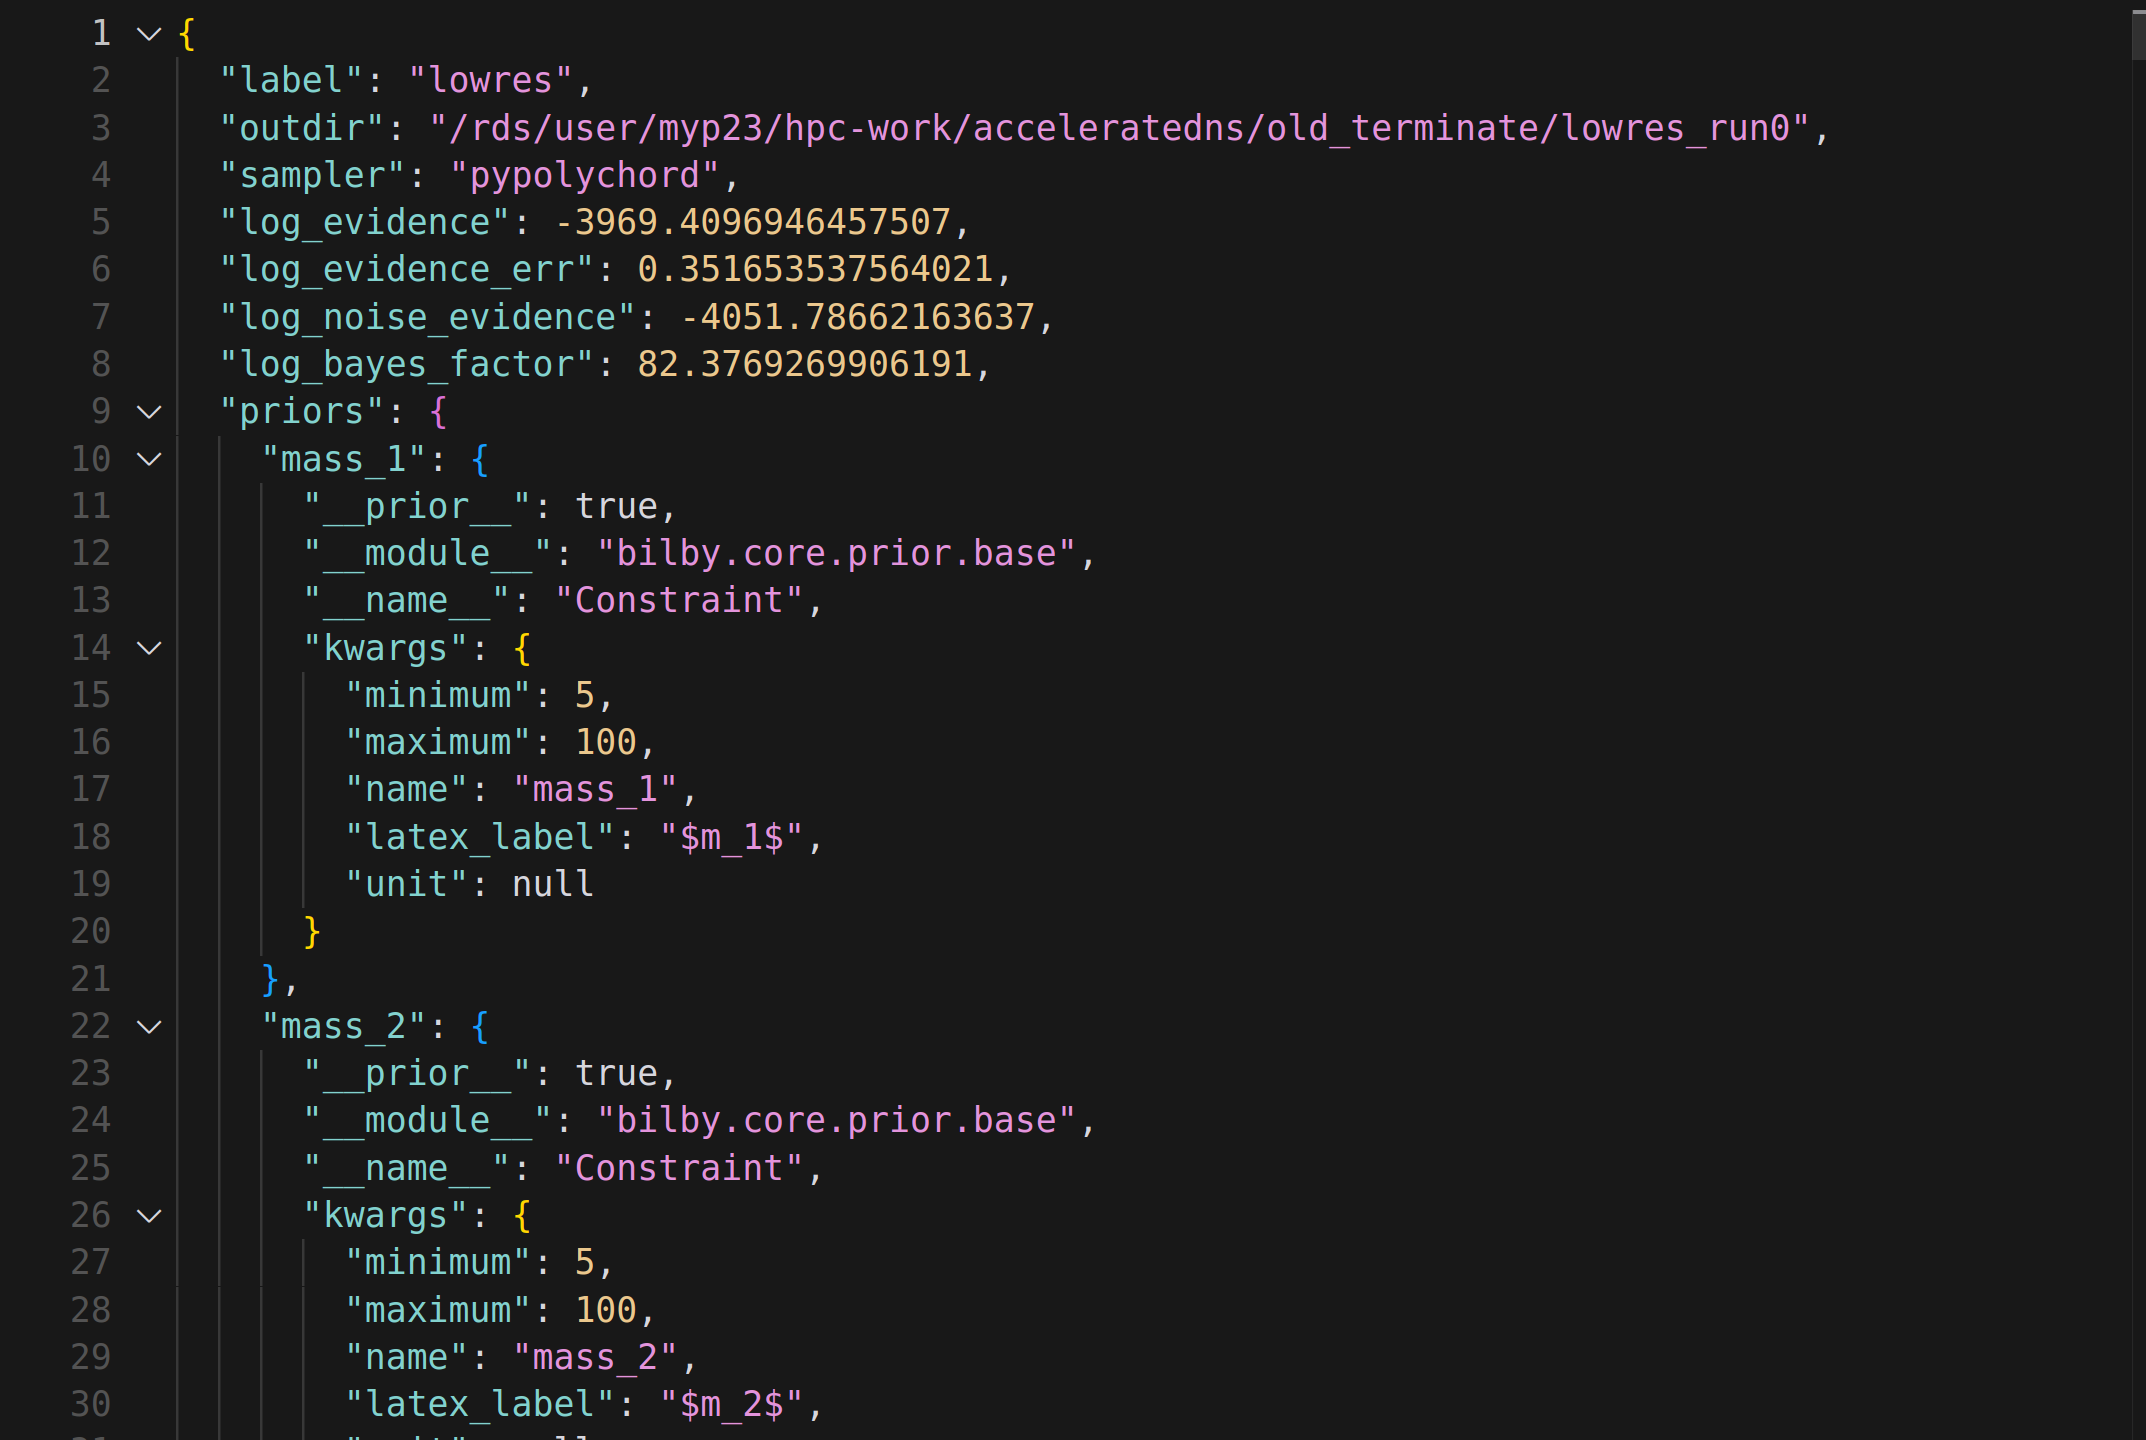
\includegraphics[width=0.95\textwidth]{Ca_Foscari Beamer/bilby_evidence.png}
    \end{minipage}%
    \begin{minipage}[]{0.5\textwidth} \vspace{2em}
        \centering
        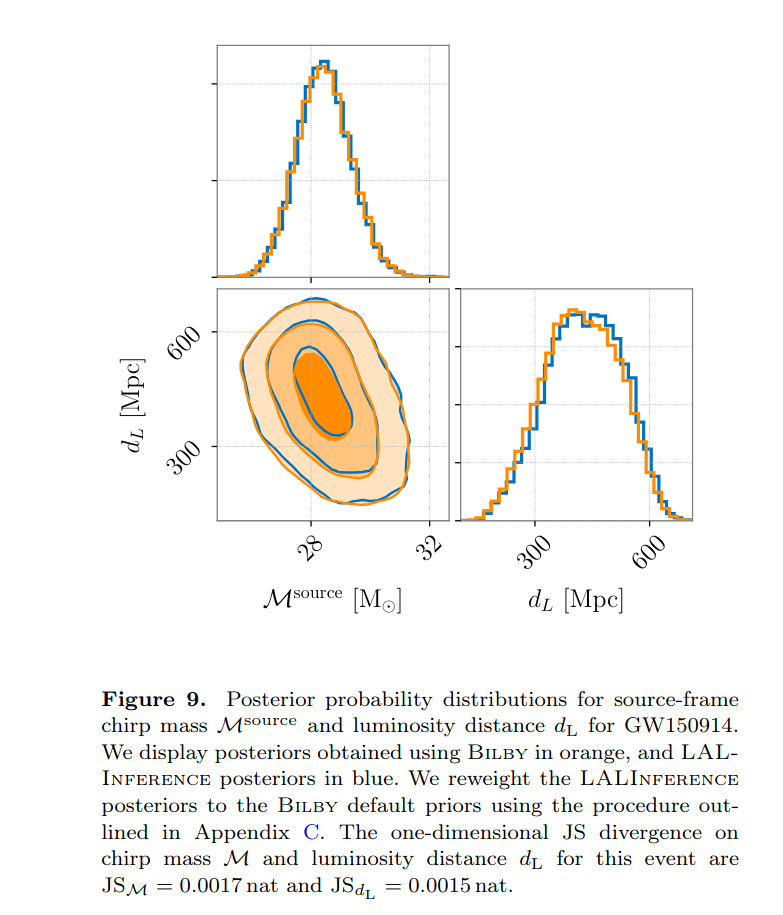
\includegraphics[width=0.75\textwidth]{Ca_Foscari Beamer/bilby_triangle.png}
    \end{minipage}
  \textcolor{cfgrey}{2006.00714}
\end{frame}

% %---------------------------------------------------------
% \begin{frame}
% \frametitle{Nested sampling (NS)}
% Nested sampling first and foremost calculates this evidence. The evidence is the integral of likelihood $\times$ prior over the entire parameter space,
% \begin{equation}
%     \mathcal{Z} = \int \mathcal{L(\theta)} \pi(\theta) d\theta,
% \end{equation}
% which, in general, is a many dimensional integral.
% \vfill

% NS turn this into a 1D problem, performing this integral by summing over nested likelihood contours in the parameter space.
% \end{frame}

%---------------------------------------------------------
%Example of the \pause command
\begin{frame}
\frametitle{Nested sampling (NS)}\vfill
Nested sampling first and foremost calculates evidence, $\mathcal{Z} = \int \mathcal{L(\theta)} \pi(\theta) d\theta$.
\begin{minipage}[]{0.35\textwidth}
\vspace{20em}
\visible<1>{
\begin{tikzpicture}
\def\svgwidth{\textwidth}
\input{NS_cartoon_2.pdf_tex}
\end{tikzpicture}
}
\visible<2>{
\begin{tikzpicture}
\def\svgwidth{\textwidth}
\hspace{-0.39cm}
\input{NS_cartoon_3.pdf_tex}
\end{tikzpicture}
}
\visible<3>{
\begin{tikzpicture}
\def\svgwidth{\textwidth}
\hspace{-0.78cm}
\input{NS_cartoon_4.pdf_tex}
\end{tikzpicture}
}
\visible<4>{
\begin{tikzpicture}
\def\svgwidth{\textwidth}
\hspace{-1.2cm}
\input{NS_cartoon_5.pdf_tex}
\end{tikzpicture}
}
\visible<5>{
\begin{tikzpicture}
\def\svgwidth{\textwidth}
\hspace{-1.6cm}
\input{NS_cartoon_5.pdf_tex}
\end{tikzpicture}
}
\vspace{-5em}
\end{minipage}\hfill
\begin{minipage}{0.5\textwidth}
    \begin{itemize}
        \item<1-> Prior is populated with set of `live points'.
        \item<2-> At each iteration $i$, point is lowest likelihood is deleted and new live point is drawn, which must have a likelihood higher than that of the deleted point.
        \item<4-> Live points compress exponentially towards peak of likelihood.
        \item<5-> Evidence is calculated as weighted sum over deleted (`dead') points.
    \end{itemize}
    %\vspace{-2.5em}
\end{minipage}
\end{frame}

%---------------------------------------------------------

\section{Accelerating NS}

%---------------------------------------------------------
%Highlighting text
% \begin{frame}{Runtime of NS}
% Time of convergence of NS:
% \vfill
%     \begin{equation}
%         T \propto \tikzmarknode{a1}{T_{\mathcal{L}}} \times \tikzmarknode{a2}{f_{\textrm{sampler}}} \times \visible<2->{\tikz\node[draw=cfred, inner sep=8.5pt, circle, overlay, shift={(10pt,2pt)}]{}} \tikzmarknode{a3}{D_{\textrm{KL}}} \times \tikzmarknode{a4}{n_{\textrm{live}}} 
%     \end{equation}
%     \begin{tikzpicture}[remember picture, overlay]
%     \visible<6>{\draw[explain, <-, thick, cfred](a4)--++(1.5,2)node[above]{resolution};}
%     \visible<4-7>{\draw[explain, <-, thick, cfred](a1)--++(-1,-0.9)node[below]{single likelihood evaluation time};}
%     \visible<5-8>{\draw[explain, <-, thick, cfred](a2)--++(-2,1)node[above]{drawing new live point subject to hard likelihood constraint};}
%     \visible<5>{}
%     \visible<3-9>{\draw[explain, <-, thick, cfred](a3)--++(.5,-2)node[below]{compression from prior to posterior ($\approx \mathrm{ln}\frac{V_\pi}{V_\mathcal{P}}$)};}
%     \visible<7->{\draw[explain, <-, thick](a4)--++(1.5,2)node[above]{resolution (baked in)};}
%     \visible<8->{\draw[explain, <-, thick](a1)--++(-1,-0.9)node[below]{faster waveform models};}
%      \visible<9->{\draw[explain, <-, thick](a2)--++(-2,1)node[above]{better samplers};}
%      \visible<2>{\draw[explain, <-, thick, cfred](a3)--++(.5,-2)node[below]{focus of this talk};}
%     \end{tikzpicture}
% \end{frame}

\begin{frame}{Runtime of NS}
Time of convergence of NS:
\vfill
\begin{equation}
    T \propto \tikzmarknode{a1}{T_{\mathcal{L}}} \times \tikzmarknode{a2}{f_{\textrm{sampler}}} \times 
    \visible<2->{\tikz\node[draw=cfred, inner sep=8.5pt, circle, overlay, shift={(10pt,2pt)}]{}} 
    \tikzmarknode{a3}{D_{\textrm{KL}}} \times \tikzmarknode{a4}{n_{\textrm{live}}} 
\end{equation}
\begin{tikzpicture}[remember picture, overlay]
    % T_L annotation
    \visible<4-7>{\draw[explain, <-, thick, cfred] (a1)--++(-1,-0.9) 
    node[below]{single likelihood evaluation time};}
    \visible<8->{\draw[explain, <-, thick] (a1)--++(-1,-0.9) 
    node[below]{faster waveform models};}
    
    % f_sampler annotation
     % Adding the image for the arrow description
    \visible<5>{\node[anchor=south, inner sep=0pt] at (current page.east) {\hspace{-20em}
        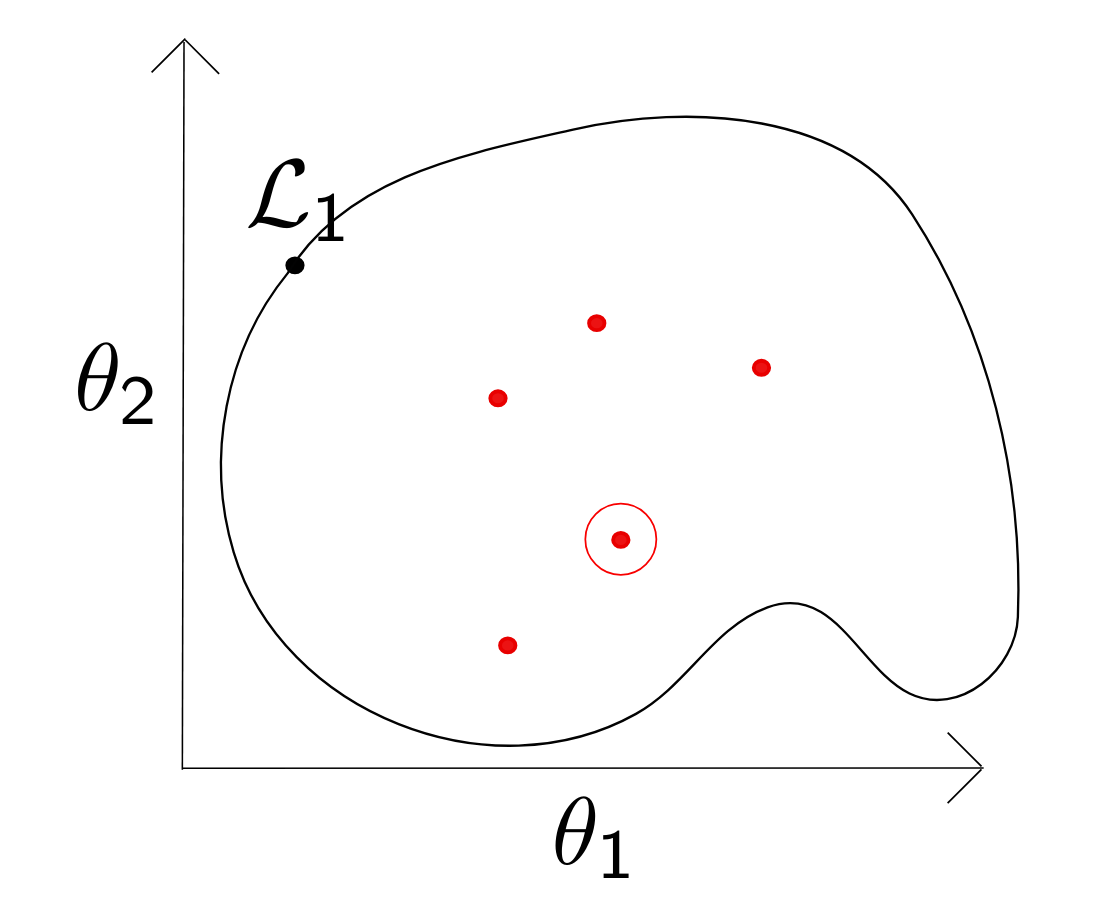
\includegraphics[width=0.2\textwidth]{Ca_Foscari Beamer/Screenshot from 2024-11-22 10-06-12.png}
    };
    }
    \visible<5-8>{\draw[explain, <-, thick, cfred] (a2)--++(-2,1) 
    node[above]{drawing new live point subject to hard likelihood constraint};}
    \visible<9->{\draw[explain, <-, thick] (a2)--++(-2,1) 
    node[above]{better samplers};}
    
    % D_KL annotation
    \visible<3-9>{\draw[explain, <-, thick, cfred] (a3)--++(.5,-2) 
    node[below]{compression from prior to posterior ($\approx \mathrm{log}\frac{V_\pi}{V_\mathcal{P}}$)};}
    \visible<2>{\draw[explain, <-, ultra thick, cfred] (a3)--++(.5,-2) 
    node[below]{focus of this talk};}

    % n_live annotation
    \visible<6>{\draw[explain, <-, thick, cfred](a4)--++(1.5,2)node[above]{resolution};}
    \visible<7->{\draw[explain, <-, thick] (a4)--++(1.5,2) 
    node[above]{resolution (baked in)};}
\end{tikzpicture}
\end{frame}

\begin{frame}{Runtime of NS}

\begin{block}{Time of convergence of NS}
    \begin{equation}
        T \propto T_{\mathcal{L}} \times f_{\textrm{sampler}} \times D_{\textrm{KL}} \times n_{\textrm{live}} 
    \end{equation}
\end{block}
\begin{block}{Uncertainty in log$\mathcal{Z}$}
    \begin{equation}
        \sigma \propto \sqrt{D_{\textrm{KL}} / n_{\textrm{live}}}
    \end{equation}
\end{block}

\alert{Precision-normalized} runtime has quadratic dependence on KL divergence. \textcolor{cfgrey}{2212.01760}
    
\end{frame}

\begin{frame}{REACH}
\vspace{2em}
One way to do this (REACH):
\vfill
\centering
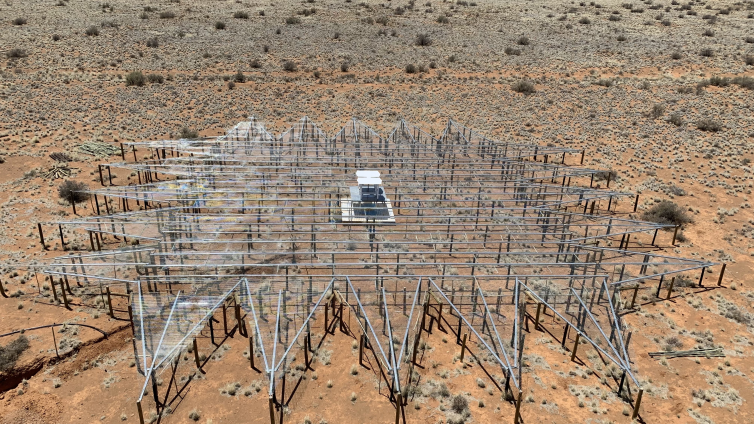
\includegraphics[width=0.6\textwidth]{Ca_Foscari Beamer/antenna.png}

\end{frame}

\begin{frame}{Reducing $D_{\textrm{KL}}$}
\vspace{3.5em}
One way to do this (REACH):

\begin{minipage}[]{0.45\textwidth}\vspace{22em}
%\includegraphics<1>[0.9\textwidth]{Ca_Foscari Beamer/antenna.png}%
\visible<1>{
\begin{tikzpicture}
\def\svgwidth{0.9\textwidth}
\input{PR_cartoon.pdf_tex}
\end{tikzpicture}
}
\visible<2>{
\begin{tikzpicture}
\def\svgwidth{0.9\textwidth}
\hspace{-0.96em}
\input{PR_cartoon_2.pdf_tex}
\end{tikzpicture}
}
\visible<3>{
\begin{tikzpicture}
\def\svgwidth{0.9\textwidth}
\hspace{-2em}
\input{PR_cartoon_3.pdf_tex}
\end{tikzpicture}
}
\end{minipage}
\begin{minipage}{0.45\textwidth}\vspace{-8em}
\begin{itemize}
    \item<1-> Perform low resolution (low live points) run first to roughly identify where posterior lies.
    \item<2-> Then set off second, high resolution, run with \textbf{narrower} box prior (much quicker).
    \item<3-> Evidence has \textbf{changed} (since different prior), but easy to correct (multiply new evidence by $\frac{V_{\pi^\ast}}{V_\pi}$)
\end{itemize}
\end{minipage}

\end{frame}


\begin{frame}{When does this break down?}\vspace{33em}
\begin{minipage}{0.6\textwidth}
   \begin{tikzpicture}
   \centering
       \def\svgwidth{\textwidth}
       \hspace{-2em}
        \input{PR_cartoon_banana.pdf_tex}
   \end{tikzpicture}
\end{minipage}
\begin{minipage}{0.3\textwidth}\vspace{-45em}
\begin{itemize}
    \item Banana distributions, multi-modality etc.
    \item Precludes its use in most realistic GW cases...
\end{itemize}
\end{minipage}
\end{frame}

\begin{frame}{NFs}
    \begin{itemize}\vspace{3em}

    \item<1-> Can iterate on this by using \textbf{normalizing flows} (NF) to learn the rough posterior.
    \item<2-> NFs perform density estimation, by learning a series of invertible mappings from the standard normal distribution to the target (posterior). 
\end{itemize}\vspace{0em}
    \visible<2->{\centering 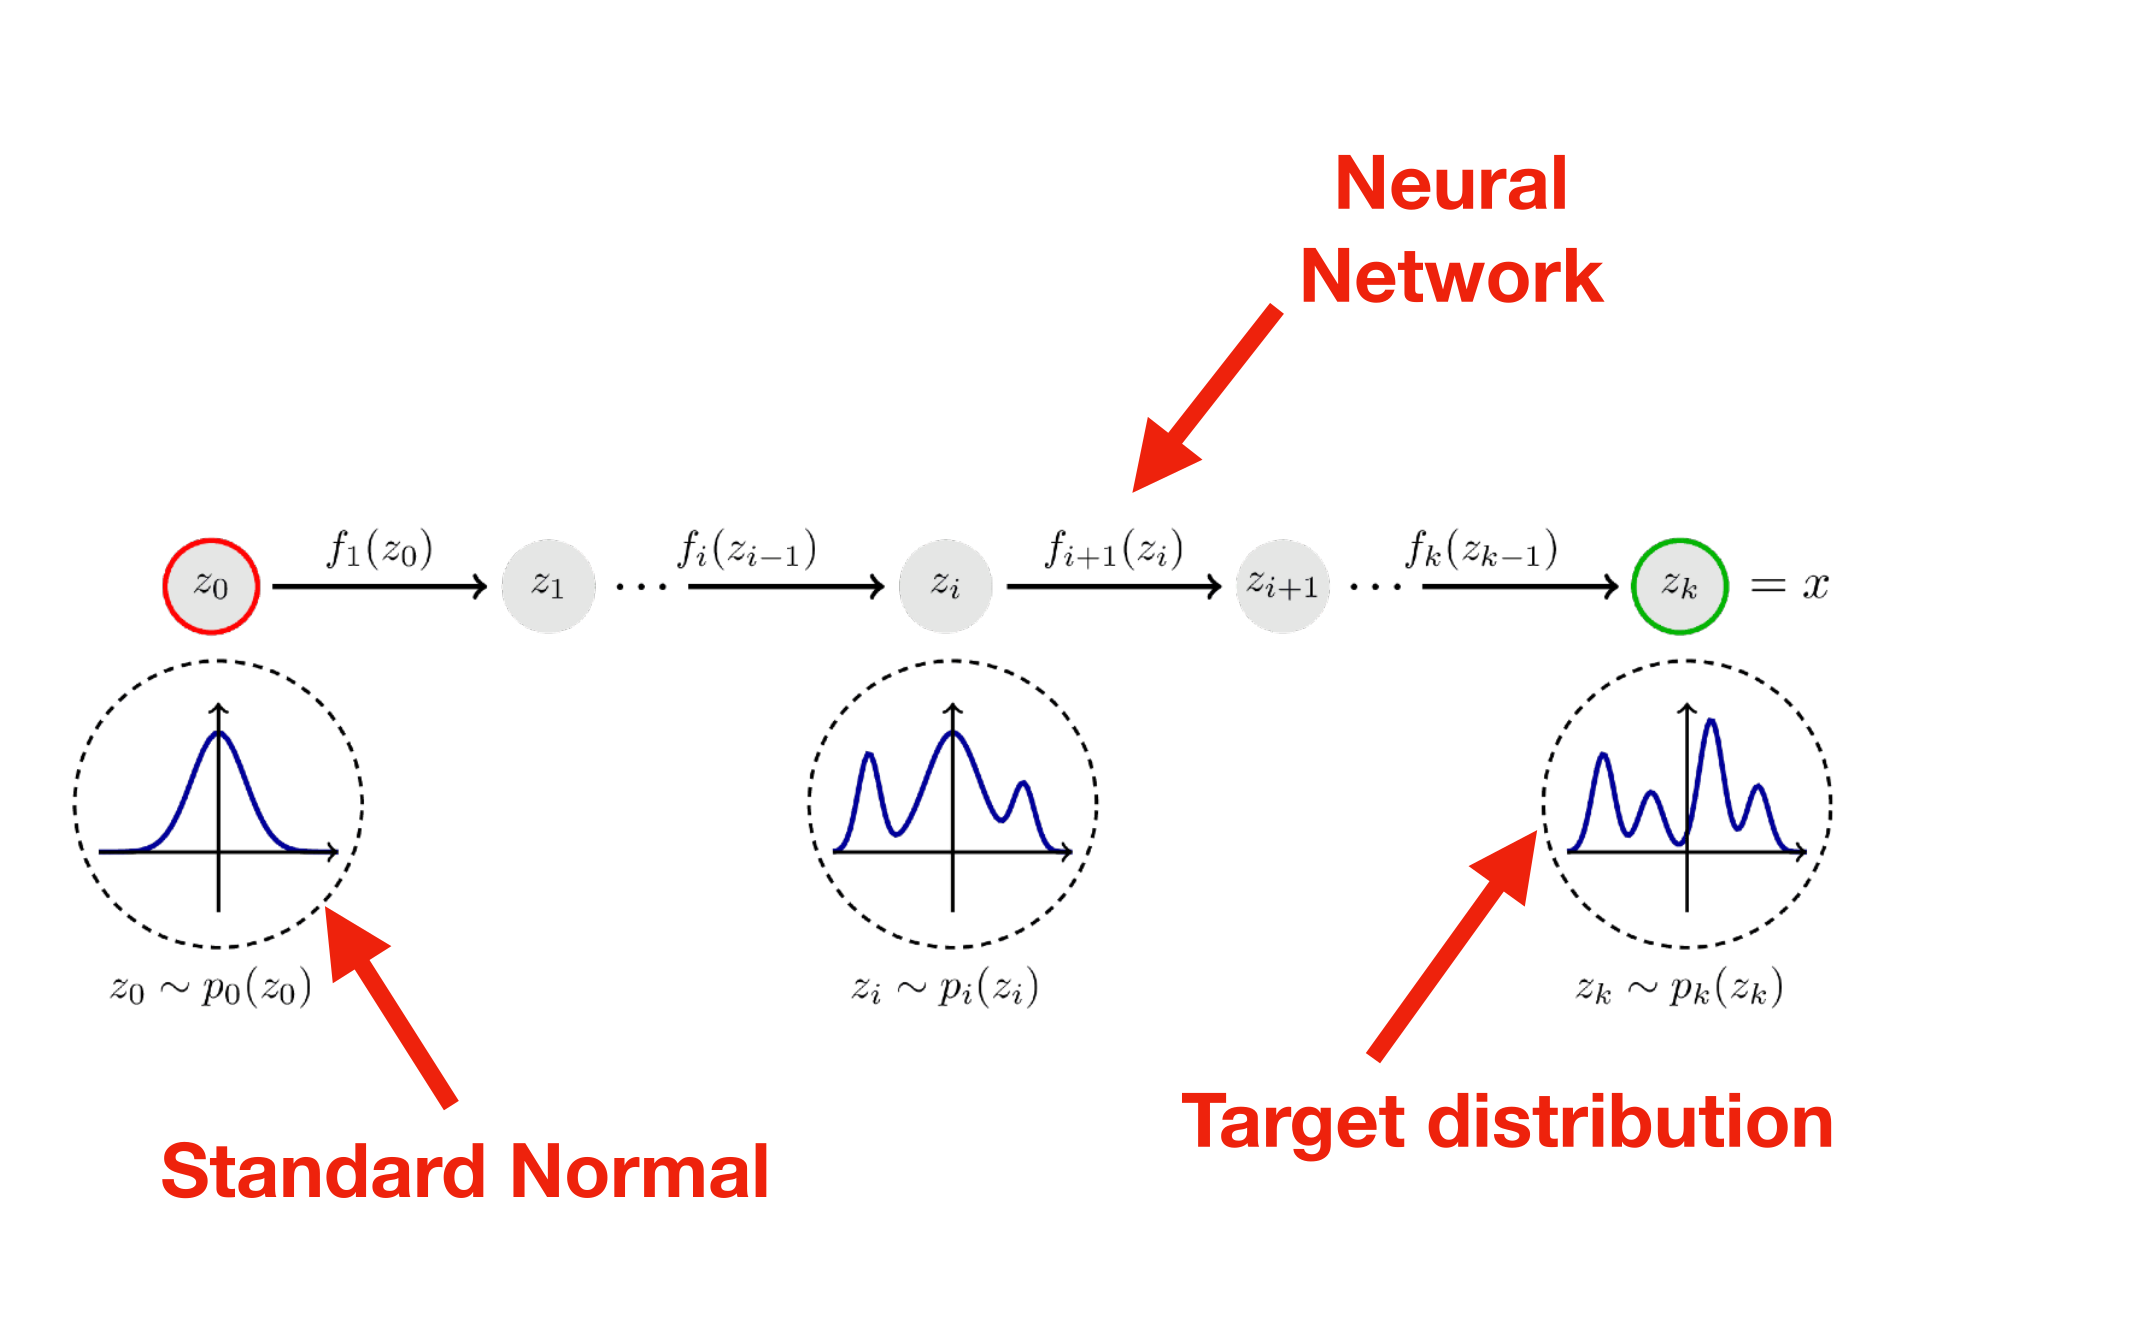
\includegraphics[width=0.5\textwidth]{Ca_Foscari Beamer/NF_diagram.png}}
\end{frame}

\begin{frame}{NF + PR}
\begin{itemize}\vspace{1em}
    \item<1-> Use \textbf{normalizing flows} (NF) to learn the rough posterior, and use this as our new prior, $\pi^\ast$.
    \item<1-> In this case, can't do our trick of correcting the second evidence by volume ratio, $\frac{V_{\pi^\ast}}{V_{\pi}}$!
    \item<1-> Must rely on another technique to get around this!
\end{itemize}\vspace{2em}
\visible<2->{\textcolor{red}{Posterior repartitioning} (PR) can help us with this - correct likelihood accordingly to get \textbf{correct} evidence out. (see e.g. \textcolor{cfgrey}{2212.01760})}\hspace{2em}\vfill
\begin{minipage}{1\textwidth}
\visible<2->{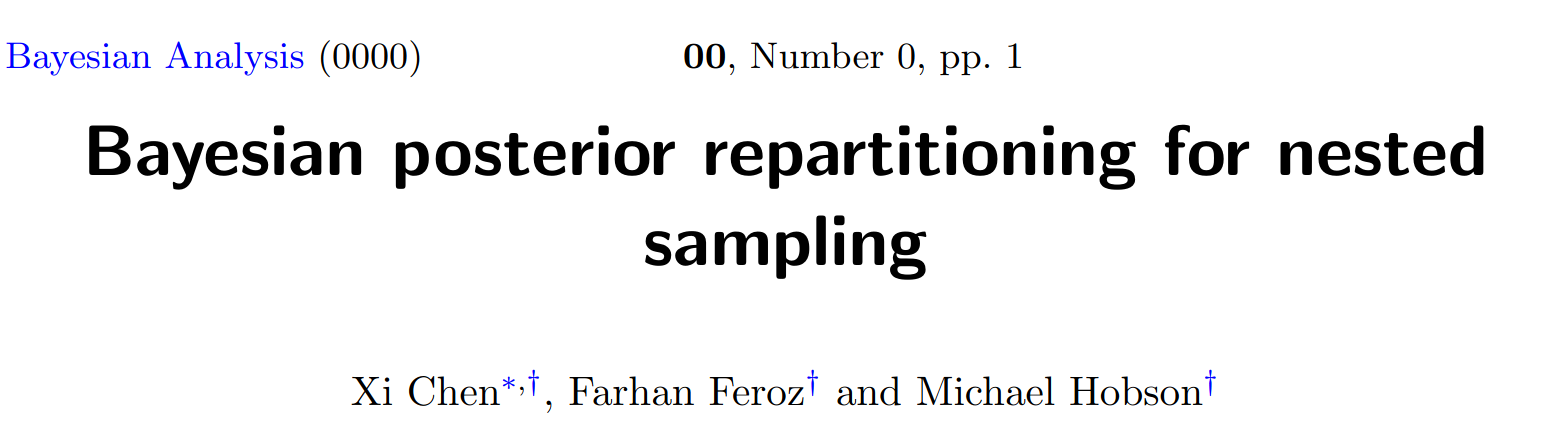
\includegraphics[width=0.3\textwidth]{Ca_Foscari Beamer/PR1.png}
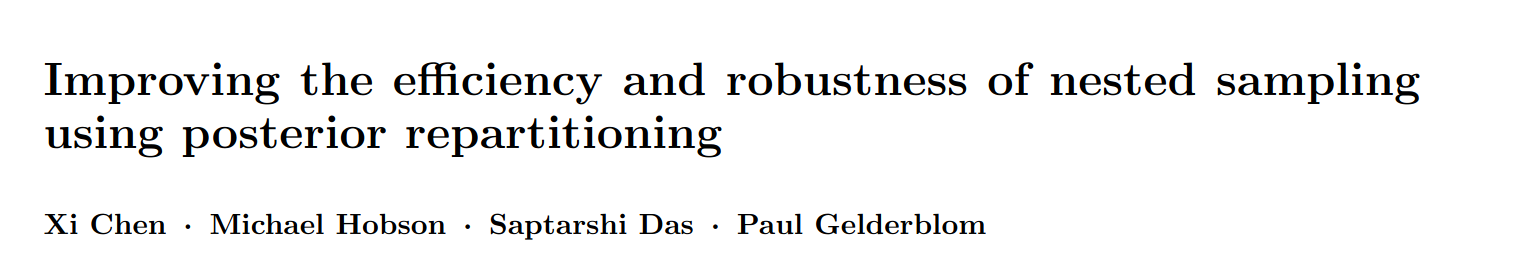
\includegraphics[width=0.38\textwidth]{Ca_Foscari Beamer/PR2.png}
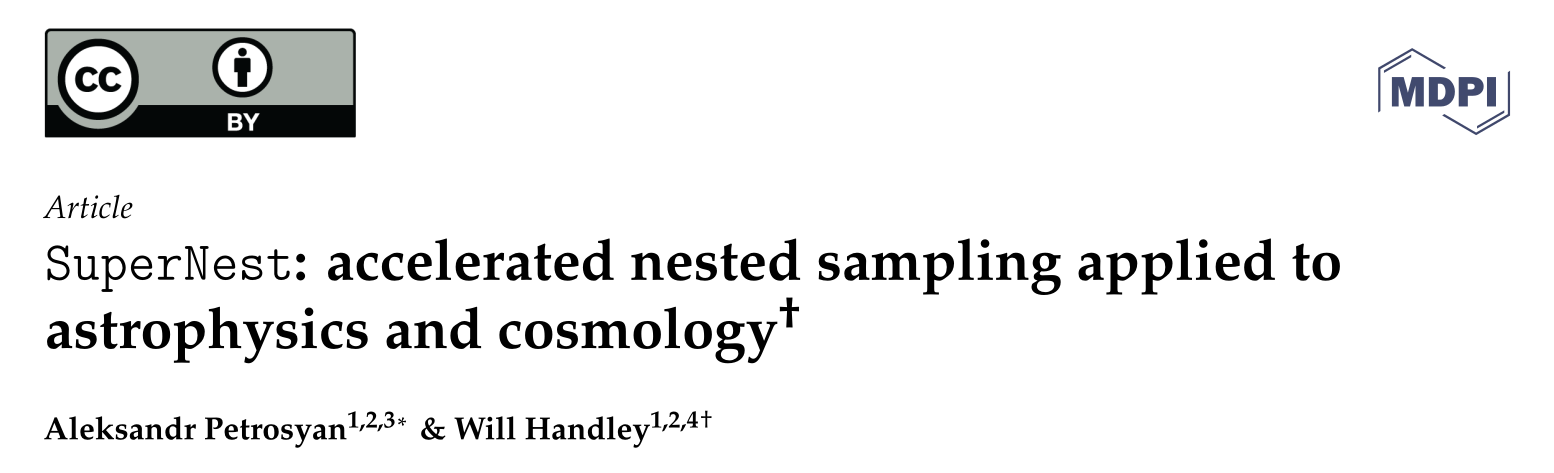
\includegraphics[width=0.3\textwidth]{Ca_Foscari Beamer/PR3.png}
}
\end{minipage}
\end{frame}

\begin{frame}{Demo on simulated example}
\begin{minipage}{0.45\textwidth}\vspace{1em}
\begin{itemize}
    \item<1-> Perform low resolution run on simulated data.
    \item<2-> Train NF on the weighted samples.
    \item<3-> Use this as `repartitioned prior' for new high resolution run (using PR to also update likelihood accordingly to same evidences and posteriors out).
\end{itemize}
\end{minipage}
\begin{minipage}{0.45\textwidth}
        \visible<1>{\vspace{2em}\begin{figure}
        \centering
        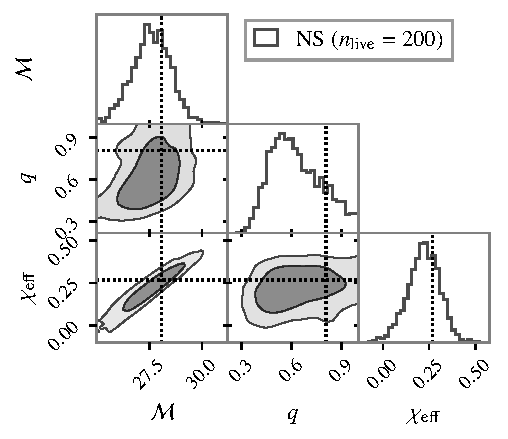
\includegraphics[width=0.9\textwidth]{Ca_Foscari Beamer/presentation_simulated_1.pdf}
    \end{figure}}
    \visible<2-3>{\vspace{-14em}\begin{figure}
        \centering
        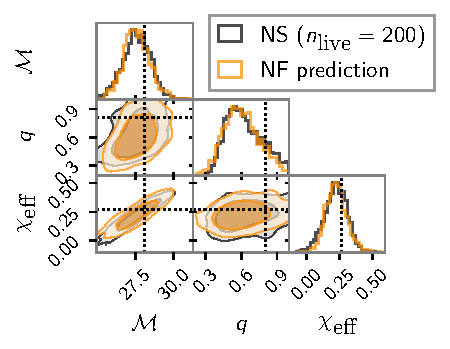
\includegraphics[width=0.9\linewidth]{Ca_Foscari Beamer/presentation_simulated_2.pdf}
    \end{figure}}
    \visible<4>{\vspace{-15em}\begin{figure}
        \centering
        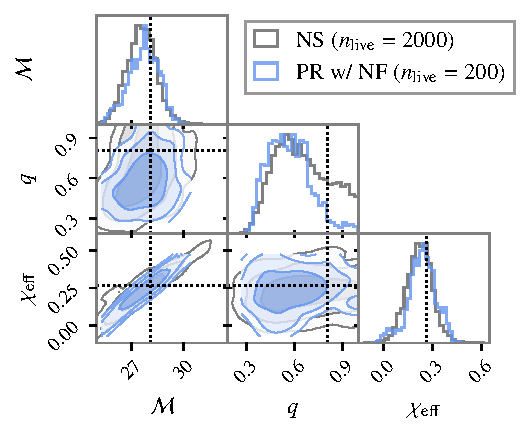
\includegraphics[width=0.9\linewidth]{Ca_Foscari Beamer/presentation_simulated_3.pdf}
    \end{figure}}
    \visible<5>{\vspace{-15em}\begin{figure}
        \centering
        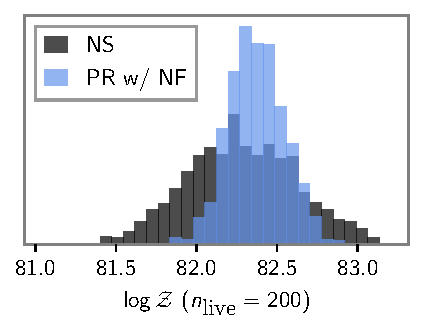
\includegraphics[width=0.9\linewidth]{Ca_Foscari Beamer/presentation_logZ_simulated.pdf}
    \end{figure}}
\end{minipage}

\vfill
\visible<5>{Same answer as doing a full resolution pass of NS, but \alert{7x faster} (precision-normalized)}.

\end{frame}

\begin{frame}{Potential pitfalls}\vfill
    \begin{itemize}
        % \item If NF learns something \textbf{narrower} than true posterior, we can make the problem harder!
        \item Still have an issue with multi-modality - if NF only learns one mode, the others can be cut off at the prior level in the high resolution run!
    \end{itemize}
    \begin{figure}
        \centering
        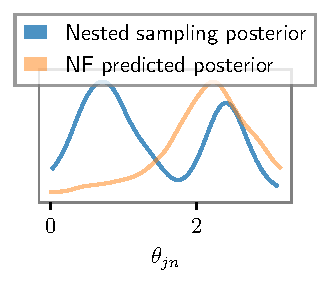
\includegraphics[width=0.4\textwidth]{Ca_Foscari Beamer/presentation_multimodality.pdf}
    \end{figure}\vspace{0em}
% \begin{itemize}
%     \item Still have an issue with multi-modality (if NF only learns one mode, the others are cut off at the prior level in the high resolution run).
% \end{itemize}
\end{frame}

\begin{frame}{Real GW example}
    When the NF has been unable to properly learn the multi-modality, we can get biased posteriors and evidences (GW191222):
 
    \begin{columns}

\column{0.5\textwidth}
\begin{figure}
    \centering
    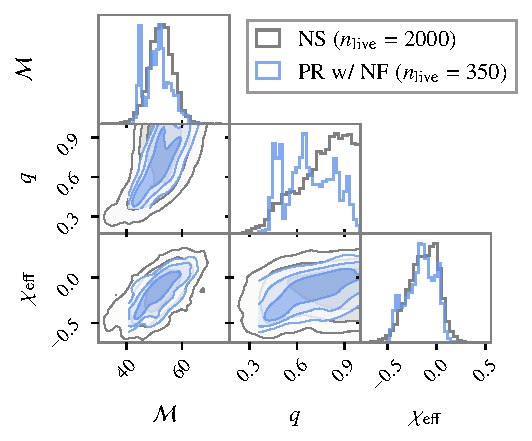
\includegraphics[width=0.75\linewidth]{Ca_Foscari Beamer/presentation_GW191222_1.pdf}
\end{figure}

\column{0.5\textwidth}
\begin{figure}
    \centering
    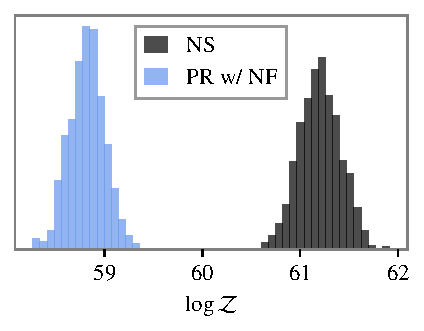
\includegraphics[width=0.75\linewidth]{Ca_Foscari Beamer/presentation_logZ_GW191222.pdf}
\end{figure}
\end{columns}
    
\end{frame}

\begin{frame}{Improving the method}
    In order to improve the robustness of the method: \vfill
    \begin{itemize}
        \item Repartitioned prior should ideally be able to \textbf{widen itself adaptively at runtime} to mitigate missed modes and badly learned posteriors.
    \end{itemize}
\end{frame}

%-----------------------------------------------------------------
\section{$\beta$-flows}

\begin{frame}{$\beta$-flows vs typical NFs}
    \begin{columns}
        \column{0.5\textwidth}\vspace{-40em}
        \begin{tikzpicture}
        \def\svgwidth{\textwidth}
        \hspace{-0em}
        \input{NS_cartoon_5.pdf_tex}
        \end{tikzpicture}
    \column{0.5\textwidth}
    \begin{itemize}
        \item Nested sampling sees tip to tail of the posterior in a systematic way, and NS has deep tails.
        \item NS can be used to train a specialized form of \textbf{conditional NFs} that can better learn these deep tail events.
        \item $\beta$-flows are new and only used in this work so far, though broadly applicable.
    \end{itemize}
    \end{columns}
\end{frame}

\begin{frame}{$\beta$-flows for PR}
\begin{columns}
\column{0.6\textwidth}
    \begin{itemize}
        \item $\beta$-flow can predict the posterior better in the tails.
        \item Can \textbf{widen themselves adaptively} at runtime.
        \item Changing a parameter $\beta$, can set repartitioned prior anywhere between posterior ($\beta=1$) and the original prior ($\beta=0$).
        % \item We use a parameter $\beta$, which is \textbf{sampled over} at runtime (same $\beta$ as in thermodynamics).
        % \item We set the helper prior to be anywhere between the posterior ($\beta=1$) and the original prior ($\beta=0$).
    \end{itemize}\vspace{2em}
    \begin{equation}
        p(\beta) \propto \mathcal{L}^\beta \pi, \hspace{2em} \beta \in [0,1]
    \end{equation}
\column{0.34\textwidth}
\begin{figure}
    \centering
    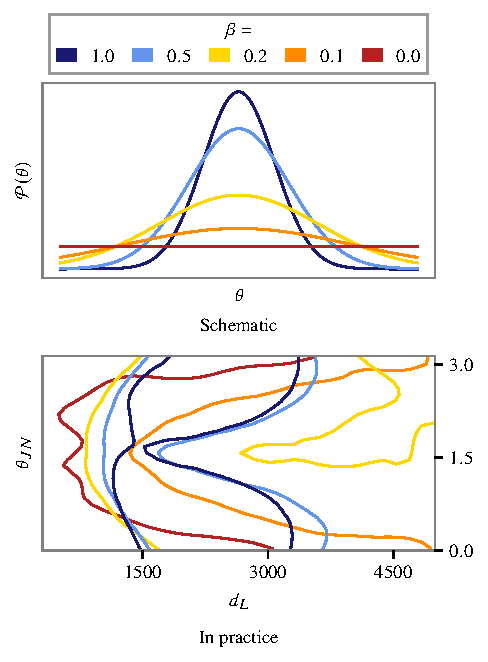
\includegraphics[width=1\textwidth]{Ca_Foscari Beamer/figure3_beta.pdf}
\end{figure}
\end{columns}   
\end{frame}

%---------------------------------------------------------
%Highlighting text
\begin{frame}
\frametitle{GW191222 (again)}
    \begin{itemize}\vspace{2em}
        \item Using $\beta$-flows to set the repartitioned prior for the high resolution run, instead of a typical NF, and sampling over $\beta$ now fixes the problem.
        \item Although $\beta$-flow also doesn't manage to learn the full multi-modality of posterior, we can preferentially sample from lower $\beta$s (i.e. wider distributions that include missed modes).
    \end{itemize}
\begin{columns}
    \column{0.3\textwidth}
        \centering
        \includegraphics<2>[width=\linewidth]{Ca_Foscari Beamer/presentation_GW191222_1.pdf}%
        \includegraphics<3->[width=\linewidth]{Ca_Foscari Beamer/presentation_GW191222_1_beta.pdf}%
    \column{0.3\textwidth}
        \centering
        \includegraphics<2>[width=\linewidth]{Ca_Foscari Beamer/presentation_GW191222_2.pdf}%
        \includegraphics<3->[width=\linewidth]{Ca_Foscari Beamer/presentation_GW191222_2_beta.pdf}%
    \column{0.3\textwidth}
        \centering
        \includegraphics<2>[width=\linewidth]{Ca_Foscari Beamer/presentation_logZ_GW191222.pdf}%
        \includegraphics<3->[width=\linewidth]{Ca_Foscari Beamer/presentation_logZ_GW191222_beta.pdf}%
\end{columns}

\visible<4>{Only \textcolor{red}{2x} (precision-normalized) as fast as normal NS for this real example, but robust.}
\end{frame}
%---------------------------------------------------------

\begin{frame}{Summary}
    \begin{itemize}
        \item<1-> Several ways to reduce NS runtime, including reducing amount of compression from prior to posterior.
        \begin{itemize}
        \item<1-> Can perform low resolution run to identify rough posterior, learn distribution with a flow, and perform high resolution run with this updated prior.
        \item<1-> Use posterior repartitioning to get correct evidences out, despite changed prior.
        \item<1-> Can achieve order of magnitude speedups on realistic GW examples.
        \end{itemize}\vfill
        \item<2-> Introduced $\beta$-flows:
        \begin{itemize}
            \item<2-> Conditional normalizing flow, trained with whole NS run
            \item<2-> Better at deep tail events
            \item<2-> First application is in this paper, but their use is much broader!
        \end{itemize}
    \end{itemize}
\end{frame}

\begin{frame}{}
    \centering
    Thank you for listening!
    \vfill
    
\includegraphics[width=0.25\textwidth]{Ca_Foscari Beamer/qr-code.png}
\end{frame}

\begin{frame}{Posterior repartitioning (PR)}
Unlike other sampling algorithms, such as Metropolis-Hastings or Hamiltonian Monte Carlo, NS distinguishes between $\mathcal{L}$ and $\pi$ by \alert{`sampling from the prior, subject to the hard likelihood constraint, $\mathcal{L}$'}.

But evidence and posteriors only depend on product of $\mathcal{L}$ and $\pi$: \vspace{-2em}
\begin{multicols}{2}
\begin{equation}
    \mathcal{Z} = \int \mathcal{L}(\theta) \pi(\theta) d\theta
\end{equation}\break
\begin{equation}
    \mathcal{P}(\theta) = \frac{\mathcal{L}(\theta)\pi(\theta)}{\mathcal{Z}}
\end{equation}
\end{multicols}
\bblock{Therefore, we are free to redefine the likelihood and prior however we like - as long as the product is the same! \textcolor{cfgrey}{arXiv:1908.04655}}
    \centering
    \begin{equation}
        \tilde{\mathcal{Z}} = \int \tilde{\mathcal{L}}(\theta) \tilde{\pi}(\theta) d\theta = \int \mathcal{L}(\theta) \pi(\theta) d\theta = \mathcal{Z}
    \end{equation}
\eblock
\end{frame}
%---------------------------------------------------------

%---------------------------------------------------------

\begin{frame}{Better at deep tail probabilities}
    \begin{columns}
        \column{0.5\textwidth}\vspace{3em}
        \begin{figure}
            \centering
            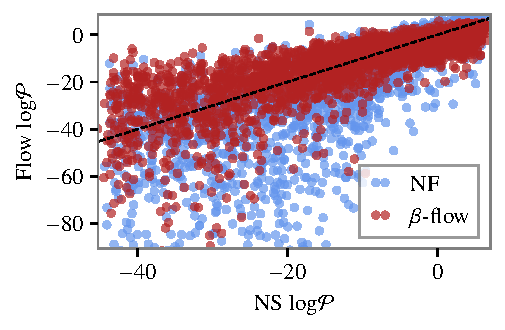
\includegraphics[width=0.9\textwidth]{Ca_Foscari Beamer/presentation_NF_vs_betaflow_simulated.pdf}
        \end{figure}
    \column{0.5\textwidth}
    \begin{itemize}
        \item For simulated example shown before, the $\beta$-flow is able to better predict the NS posterior probabilities.
        \item $\beta$-flows exhibit less scatter in the tails (low posterior probabilities) than the NFs.
    \end{itemize}
    \end{columns}
\end{frame}

\begin{frame}{What is $\beta$?}
\begin{itemize}\vspace{2em}
    \item NS compresses step by step from prior to posterior.
    \item We can label these stages by a parameter $\beta$ (akin to inverse temperature $\beta$ in e.g. materials science). 
    \item Sliding scale from $\beta = 0$ as the prior and $\beta = 1$ as the posterior.
\end{itemize}
\begin{figure}
    \centering
    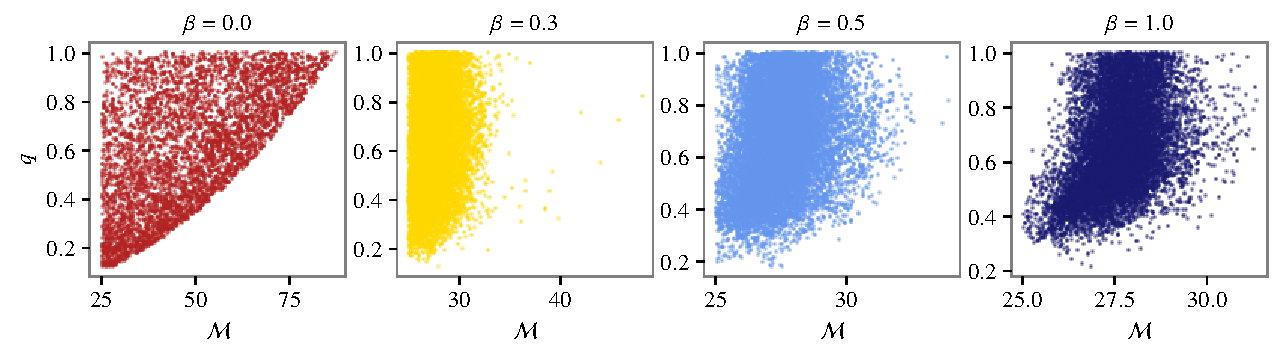
\includegraphics[width=0.9\linewidth]{Ca_Foscari Beamer/presentation_beta.pdf}
\end{figure}

\end{frame}

\begin{frame}{Adaptive proposal}
\begin{columns}
\column{0.7\textwidth}
    \begin{itemize}
        \item $\beta$-flow can predict the ($\beta = 1$) posterior, similarly to NF (but better in tails).
        \item Can predict \textbf{any intermediate stage} of NS too.
        \item We \textbf{sample over $\beta$} at runtime, so proposal can now widen itself adaptively if modes have been missed!
    \end{itemize}
\column{0.3\textwidth}
\begin{figure}
    \centering
    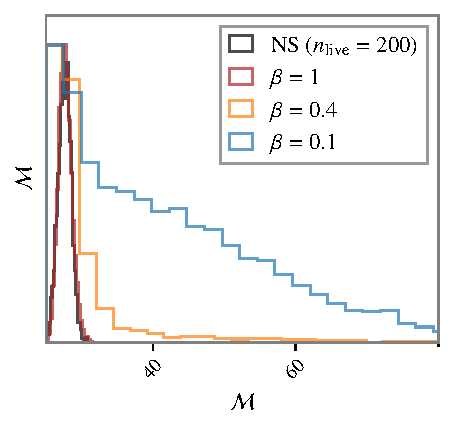
\includegraphics[width=1\textwidth]{Ca_Foscari Beamer/presentation_beta_1.pdf}
\end{figure}
\end{columns}   
\end{frame}

\end{document}